\documentclass[10pt,twocolumn]{article}
\usepackage[T1]{fontenc}
\usepackage{lmodern}
\usepackage[margin=0.58in,columnsep=0.22in]{geometry}
\usepackage{amsmath,amssymb,mathtools,bm}
\usepackage{tikz}
\usetikzlibrary{arrows.meta,positioning,calc}
\usepackage{xcolor}
\usepackage{microtype}
\usepackage[colorlinks=true,linkcolor=blue!50!black,urlcolor=blue!50!black,citecolor=blue!50!black]{hyperref}

\setlength{\parindent}{0pt}
\setlength{\parskip}{1.5pt}
\setlength{\abovedisplayskip}{4pt}
\setlength{\belowdisplayskip}{4pt}
\setlength{\abovedisplayshortskip}{3pt}
\setlength{\belowdisplayshortskip}{3pt}
\allowdisplaybreaks
\sloppy
\raggedbottom

\newcommand{\ket}[1]{|#1\rangle}
\newcommand{\bra}[1]{\langle #1|}
\newcommand{\micro}[1]{\par\noindent\textbf{Micro-intuition:}\ #1\par}
\newcommand{\form}[1]{\par\noindent\textbf{Common mathematical form:}\ #1\par}
\newcommand{\commentary}[1]{\par\noindent\textbf{Commentary:}\ #1\par}
\newcommand{\phys}[1]{\par\noindent\textbf{Quantum-mechanical interpretation:}\ #1\par}
\newcommand{\geom}[1]{\par\noindent\textbf{Geometric visualization:}\ \textcolor{teal!70!black}{#1}\par}
\newcommand{\conceptbreak}{\par\medskip\noindent{\color{black!30}\rule{\columnwidth}{0.35pt}}\par\medskip}
\newenvironment{insight}{\begin{center}\begin{minipage}{0.94\columnwidth}\color{blue!35!black}\textbf{Structural checkpoint.}\ }{\end{minipage}\end{center}}

\title{Formal-Manifold Propagation After Batch Admission\\
\large Supported Tangents, Trust, Transport, and Recycled Response}
\author{}
\date{}

\begin{document}
\maketitle
\vspace{-1.3em}

This note begins where \emph{Joint Metric--Schur Batch Selection} ends. The
metric--Schur prune note has already established projection, supported
pseudoinversion, regularized response, and rollback-safe deletion. The batching
note has already established joint old--new Gram and Hessian blocks, Schur
relaxation, batch novelty, and a metric trust constraint. Those derivations are
reused rather than taught again.

The new question is temporal in the optimization sense. Once a singleton or
batch has been admitted, how can the accepted ansatz be reoptimized through a
sequence of nearby quantum states while gradients, metrics, and learned
curvature continue to describe compatible tangent spaces?

\section*{Prerequisite Entrance Exam}

This detachable exam draws only from \emph{Metric-Regularized Schur Prune
Response} and \emph{Joint Metric--Schur Batch Selection}, in that reading
order. Choose the strongest answer and record why it beats the nearest
alternative. The labeled answer key is in the final solutions section.

\subsection*{Conceptual Judgment}

\textbf{1. Gram information.}
What does the Fubini--Study Gram matrix determine for a real coordinate step
\(p\)?

\textbf{A.} Its exact finite energy decrease.\quad
\textbf{B.} Its compiled circuit depth.\quad
\textbf{C.} The squared length of its horizontal physical tangent.\quad
\textbf{D.} The number of nonzero generator coefficients.

\textbf{2. Support selection and ridge damping.}
Which statement preserves the distinction developed in the prerequisite
notes?

\textbf{A.} A ridge declares the physical quotient rank, while support
selection changes only step magnitude.\quad
\textbf{B.} Support selection declares the resolved quotient; a ridge modifies
the response assigned within that declared support.\quad
\textbf{C.} Both operations delete ansatz generators from the circuit.\quad
\textbf{D.} Both operations are equivalent whenever the matrix is symmetric.

\textbf{3. Schur elimination.}
What happens to the old-coordinate block in a joint batch model?

\textbf{A.} Its stationary response as a function of the batch amplitudes is
solved and substituted into the reduced model.\quad
\textbf{B.} Its coordinates are physically deleted before the batch is
scored.\quad
\textbf{C.} Its Hessian block is replaced by its Gram block.\quad
\textbf{D.} Its amplitudes are set to zero throughout the local model.

\textbf{4. Joint response.}
Two candidates have favorable singleton scores. When does their sum describe
the batch response?

\textbf{A.} Whenever both raw gradients have the same sign.\quad
\textbf{B.} Whenever their individual Gram norms agree.\quad
\textbf{C.} Whenever they originate from different parent records.\quad
\textbf{D.} When the joint metric and Hessian cross-couplings make the reduced
response effectively additive.

\textbf{5. Residual rank.}
One eigenvalue of the residual batch Gram matrix vanishes after quotienting by
the active tangent span. What follows?

\textbf{A.} The entire batch has zero energy gradient.\quad
\textbf{B.} One collective candidate combination supplies no resolved new
physical tangent direction at the current ray.\quad
\textbf{C.} The energy Hessian has the same null eigenvector.\quad
\textbf{D.} Every candidate in the batch must be removed individually.

\textbf{6. Metric trust.}
What does the constraint \(p^{\mathsf T}Gp\leq\rho^2\) limit?

\textbf{A.} The Euclidean size of the raw parameter array in every chart.\quad
\textbf{B.} The predicted energy curvature along the batch.\quad
\textbf{C.} The local physical state displacement measured by the tangent
metric.\quad
\textbf{D.} The number of candidates admitted in one batch.

\subsection*{Terminology and High-Level Vocabulary}

\textbf{7. Positive semidefinite Gram form.}
What conclusion is licensed by calling \(G\) positive semidefinite?

\textbf{A.} Every eigenvalue of \(G\) is strictly positive.\quad
\textbf{B.} The quadratic form satisfies \(p^{\mathsf T}Gp\geq0\) for every
real \(p\), while null directions may remain.\quad
\textbf{C.} Every coordinate direction is physically independent.\quad
\textbf{D.} The energy decreases for every nonzero coordinate step.

\textbf{8. Coordinate quotient.}
What is identified in \(\mathbb R^d/\ker T\)?

\textbf{A.} Candidate sets with equal resource cost.\quad
\textbf{B.} Energy models with equal Hessian eigenvalues.\quad
\textbf{C.} Quantum states with equal variational energy.\quad
\textbf{D.} Coordinate arrays whose difference produces no horizontal
physical tangent.

\textbf{9. Schur complement.}
What mathematical operation earns this name in the local quadratic model?

\textbf{A.} Solving one block's stationary response and substituting it into
the remaining block.\quad
\textbf{B.} Projecting every negative eigenvalue to zero.\quad
\textbf{C.} Diagonalizing the Gram and Hessian simultaneously.\quad
\textbf{D.} Multiplying the batch gain by a novelty score.

\textbf{10. Batch nonadditivity.}
What does nonadditivity report?

\textbf{A.} The batch violates a circuit-symmetry rule.\quad
\textbf{B.} Every singleton in the batch has negative predicted gain.\quad
\textbf{C.} Cross-couplings make the joint reduced response differ from the
sum of isolated singleton responses.\quad
\textbf{D.} The batch contains a Gram-null direction.

\subsection*{Mathematical-Form Recognition}

\textbf{11. Pulled-back physical length.}
Let \(T\) map real coordinate steps into horizontal tangents and let
\(G=\Re(T^*T)\). Which identity identifies the Gram quadratic form?
\[
\begin{aligned}
\mathrm{A}\quad&p^{\mathsf T}Gp=\|Gp\|_2^2,\\
\mathrm{B}\quad&p^{\mathsf T}Gp=\|Tp\|_{\mathbb R}^2,\\
\mathrm{C}\quad&p^{\mathsf T}Gp=\operatorname{tr}(T),\\
\mathrm{D}\quad&p^{\mathsf T}Gp=p^{\mathsf T}Hp.
\end{aligned}
\]

\textbf{12. Supported pseudoinverse.}
Let \(G V=V\Lambda\), where the columns of \(V\) are the retained orthonormal
eigenvectors and \(\Lambda\succ0\) contains their eigenvalues. Which expression
is the Moore--Penrose inverse on this support?
\[
\begin{aligned}
\mathrm{A}\quad&G^+=V^{\mathsf T}\Lambda^{-1}V,\\
\mathrm{B}\quad&G^+=V\Lambda V^{\mathsf T},\\
\mathrm{C}\quad&G^+=V^{\mathsf T}\Lambda V,\\
\mathrm{D}\quad&G^+=V\Lambda^{-1}V^{\mathsf T}.
\end{aligned}
\]

\textbf{13. Schur-reduced quadratic form.}
Let
\[
q(x,y)=\tfrac12x^{\mathsf T}Ax+x^{\mathsf T}By
+\tfrac12y^{\mathsf T}Cy,
\]
and suppose the supported stationary response is
\(x^*(y)=-A^+By\). Which matrix governs the reduced quadratic in \(y\)?
\[
\begin{aligned}
\mathrm{A}\quad&C-B^{\mathsf T}A^+B,\\
\mathrm{B}\quad&C+B^{\mathsf T}A^+B,\\
\mathrm{C}\quad&A-B C^+B^{\mathsf T},\\
\mathrm{D}\quad&A+B C^+B^{\mathsf T}.
\end{aligned}
\]

\textbf{14. Coordinate-invariant trust length.}
Suppose \(p_\theta=Sp_\phi\) and
\(G_\phi=S^{\mathsf T}G_\theta S\). Which identity preserves the physical
trust boundary?
\[
\begin{aligned}
\mathrm{A}\quad&p_\phi^{\mathsf T}G_\theta p_\phi
=p_\theta^{\mathsf T}G_\phi p_\theta,\\
\mathrm{B}\quad&p_\phi^{\mathsf T}p_\phi
=p_\theta^{\mathsf T}p_\theta,\\
\mathrm{C}\quad&p_\phi^{\mathsf T}G_\phi p_\phi
=p_\theta^{\mathsf T}G_\theta p_\theta,\\
\mathrm{D}\quad&G_\phi=S^{-1}G_\theta S.
\end{aligned}
\]

\clearpage
\section*{1. The Bridge: Selection Ends, Propagation Begins}

\micro{Batching chooses a structural enlargement; propagation moves on the
accepted enlarged variational manifold.}

Paper-I notation writes the accepted ordered ansatz as
\begin{align}
\ket{\psi_k}
&=U_k(\bm\theta_k)\ket{\phi_0},
\label{eq:accepted-state}\\
U_{k+1}(\bm\theta_{k+1})
&=U_k(\bm\theta_k)\oplus\bigcup_{r\in B}r.
\label{eq:accepted-growth}
\end{align}
The batch coordinates are initialized at zero. Consequently,
\begin{equation}
U_{k+1}(\bm\theta_k,0)\ket{\phi_0}
=U_k(\bm\theta_k)\ket{\phi_0}.
\label{eq:zero-growth-state}
\end{equation}
Equation~\eqref{eq:zero-growth-state} identifies the initial physical ray, but
it enlarges the set of infinitesimal directions available at that ray. The
subsequent inner iterates are
\begin{equation}
x_j=[\psi_j],
\qquad
\ket{\psi_j}=U_{k+1}(\bm\theta_j)\ket{\phi_0},
\label{eq:inner-rays}
\end{equation}
where square brackets denote the projective ray and \(j\) indexes accepted
reoptimization steps on the fixed enlarged ansatz.

\form{This is optimization on a changing family of tangent spaces
\(T_{x_j}\mathcal M\), with discrete manifold changes at growth or pruning.}

\commentary{The outer SNAKE step changes which circuit coordinates exist. The
inner Formal-Manifold step changes the physical ray represented by those
coordinates. The state can remain unchanged at the instant of zero-coordinate
growth while its available tangent space becomes larger. This is the first
reason state identity and optimizer-state identity must be kept separate.}

\phys{The quantum system is represented by one normalized state ray before and
immediately after zero-coordinate insertion. The admitted generators supply
new possible coherent deformations of that ray. Reoptimization then chooses a
combination of inherited and newly admitted deformations that lowers the energy.
The route therefore propagates a variational state through projective Hilbert
space while occasionally changing the manifold on which that propagation is
allowed to occur.}

\geom{Picture the old ansatz as a tangent sheet touching the projective-state
surface. Zero-coordinate growth leaves the contact point fixed and unfolds
additional tangent arrows. Inner optimization then moves the contact point;
the tangent sheet tilts as it follows the curved state surface.}

\begin{center}
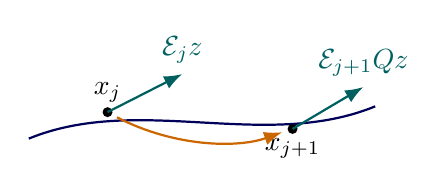
\begin{tikzpicture}[x=1cm,y=0.82cm,>=Latex]
  \draw[thick,blue!35!black] (-2.2,-0.25) .. controls (-0.8,0.45) and (0.8,-0.45) .. (2.2,0.25);
  \fill[black] (-1.2,0.16) circle (1.8pt) node[above] {$x_j$};
  \fill[black] (1.15,-0.10) circle (1.8pt) node[below] {$x_{j+1}$};
  \draw[->,teal!75!black,thick] (-1.2,0.16) -- (-0.25,0.75) node[above] {$\mathcal E_j z$};
  \draw[->,teal!75!black,thick] (1.15,-0.10) -- (2.05,0.55) node[above] {$\mathcal E_{j+1}Qz$};
  \draw[->,orange!80!black,thick] (-1.08,0.08) .. controls (-0.35,-0.38) and (0.45,-0.4) .. (1.02,-0.15);
\end{tikzpicture}
\end{center}

\conceptbreak

\section*{2. The Physical Tangent Quotient}

\micro{Different parameter arrays can describe the same infinitesimal physical
motion; the optimizer should act on the motion rather than the redundant
labels.}

At \(x_j=[\psi_j]\), define the horizontal tangent columns
\begin{align}
\Pi_j&=I-\ket{\psi_j}\bra{\psi_j},
\label{eq:horizontal-projector}\\
\ket{t_{j,a}}&=\Pi_j\partial_a\ket{\psi_j},
\label{eq:horizontal-tangent}\\
T_jp&=\sum_a p_a\ket{t_{j,a}},
\qquad p\in\mathbb R^{d_j}.
\label{eq:tangent-map}
\end{align}
The real Fubini--Study Gram matrix inherited from the earlier primers is
\begin{align}
(G_j)_{ab}
&=\Re\langle t_{j,a}|t_{j,b}\rangle,
\label{eq:fs-gram}\\
p^{\mathsf T}G_jp
&=\|T_jp\|_{\mathbb R}^2.
\label{eq:gram-pullback}
\end{align}
Therefore
\begin{equation}
p\in\ker G_j
\Longleftrightarrow
T_jp=0.
\label{eq:null-equivalence}
\end{equation}
The physical tangent space is \(\operatorname{ran}T_j\), while the independent
coordinate object is the quotient
\begin{equation}
\mathbb R^{d_j}/\ker T_j
=\mathbb R^{d_j}/\ker G_j.
\label{eq:coordinate-quotient}
\end{equation}

\form{Equation~\eqref{eq:coordinate-quotient} is a quotient space: coordinate
arrays differing by a null combination represent the same physical tangent.}

\commentary{The equivalence class is operational. Starting from one coordinate
step \(p\), every array \(p+n\) with \(n\in\ker G_j\) produces the same
horizontal state derivative. The quotient retains that common physical motion
and forgets which redundant representative produced it. Singularity is therefore
geometric information before it is an inversion problem.}

\phys{A null coordinate combination does not create an additional way for the
quantum state to move. It may correspond to duplicated generators, a local
parameter symmetry, or a direction that changes only the unphysical state
representative. Treating it as an independent response channel would let the
optimizer assign arbitrary coefficients to motion that the state cannot
realize.}

\geom{Draw two parameter arrows whose images under \(T_j\) land on the same
tangent arrow. Their difference lies along a collapsed coordinate direction.
The quotient folds that collapsed direction to one point while preserving the
actual arrow on the state manifold.}

\conceptbreak

\clearpage
\section*{2A. From the Raw Gram Matrix to a Supported Frame}

This inserted bridge is designed to be printed independently. It begins from
Eqs.~\eqref{eq:tangent-map}--\eqref{eq:coordinate-quotient}, constructs every
object used at the start of Section~3, and ends with the representation rules
needed for parameter rescaling, gradients, curvature, and later frame
transport.

\subsection*{2A.1 Three spaces and the meaning of a frame}

\micro{A frame is an ordered collection of basis arrows; its coefficient array
records how those arrows are combined.}

At accepted inner iterate \(j\), three spaces appear:
\begin{align}
\mathbb R^{d_j}
&\xrightarrow{\ T_j\ }
\operatorname{ran}T_j
\subset T_{x_j}\mathcal M,
\label{eq:bridge-coordinate-to-tangent}\\
\mathbb R^{r_j}
&\xrightarrow{\ \mathcal E_j\ }
\operatorname{ran}T_{j,+}.
\label{eq:bridge-frame-to-tangent}
\end{align}
The space \(\mathbb R^{d_j}\) contains raw parameter-coordinate arrays. The
space \(T_{x_j}\mathcal M\) is the tangent space of the variational state
manifold at the projective state \(x_j=[\psi_j]\). The integer \(r_j\leq d_j\)
is the number of retained physical tangent modes. The map \(\mathcal E_j\)
will carry Euclidean coefficients in \(\mathbb R^{r_j}\) into an orthonormal
physical tangent basis.

A frame for an \(r\)-dimensional real inner-product space is an ordered list
of \(r\) linearly independent vectors. Writing those vectors as matrix columns
gives
\begin{equation}
\mathcal E=
\begin{bmatrix}
e_1&e_2&\cdots&e_r
\end{bmatrix}.
\label{eq:bridge-frame-definition}
\end{equation}
The frame is orthonormal when
\begin{equation}
\mathcal E^*\mathcal E=I_r,
\qquad
\langle e_a,e_b\rangle_{\mathbb R}=\delta_{ab}.
\label{eq:bridge-orthonormal-frame-definition}
\end{equation}
Here \(\mathcal E^*\) is the adjoint, \(I_r\) is the \(r\times r\) identity,
and \(\delta_{ab}\) is the Kronecker delta. A coefficient vector
\(z=(z_1,\ldots,z_r)^{\mathsf T}\) synthesizes the physical tangent
\begin{equation}
\xi=\mathcal Ez=\sum_{a=1}^{r}z_ae_a.
\label{eq:bridge-frame-synthesis}
\end{equation}

\commentary{The columns of \(V_j\) introduced below form a frame inside raw
parameter-coordinate space. The columns of \(\mathcal E_j\) form a frame
inside the physical tangent space. These matrices have different codomains.
The factors \(T_j\) and \(\Lambda_j^{-1/2}\) convert the first frame into the
second.}

\phys{A raw circuit parameter labels a control convention. A physical tangent
arrow describes an infinitesimal change of the quantum ray. The tangent map
converts the former into the latter. Whitening selects independent physical
motions and assigns them unit tangent length, producing a frame in which an
optimizer can compare response components without inheriting arbitrary angle
units.}

\geom{Picture a coordinate grid painted beneath a tangent plane. The columns
of \(V_j\) are selected directions in the painted grid. Applying \(T_j\)
raises them into physical arrows on the tangent plane. Dividing each arrow by
its length produces the orthonormal arrows stored in \(\mathcal E_j\).}

\conceptbreak

\subsection*{2A.2 The Gram matrix as a quadratic physical-length map}

\micro{The Gram matrix converts any real parameter mixture into the squared
length of the physical tangent generated by that mixture.}

For \(p=(p_1,\ldots,p_{d_j})^{\mathsf T}\in\mathbb R^{d_j}\),
Eqs.~\eqref{eq:tangent-map} and \eqref{eq:fs-gram} give
\begin{align}
T_jp
&=\sum_{a=1}^{d_j}p_a\ket{t_{j,a}},
\label{eq:bridge-tangent-mixture}\\
\|T_jp\|_{\mathbb R}^2
&=\Re\left\langle
\sum_{a=1}^{d_j}p_at_{j,a}
\middle|
\sum_{b=1}^{d_j}p_bt_{j,b}
\right\rangle,
\label{eq:bridge-length-expand-1}\\
&=\sum_{a=1}^{d_j}\sum_{b=1}^{d_j}
p_ap_b\Re\langle t_{j,a}|t_{j,b}\rangle,
\label{eq:bridge-length-expand-2}\\
&=\sum_{a=1}^{d_j}\sum_{b=1}^{d_j}
p_a(G_j)_{ab}p_b,
\label{eq:bridge-length-expand-3}\\
&=p^{\mathsf T}G_jp.
\label{eq:bridge-length-expand-4}
\end{align}
Equation~\eqref{eq:bridge-length-expand-4} makes \(G_j\) a positive-semidefinite
quadratic form. For every \(p\in\mathbb R^{d_j}\),
\begin{equation}
p^{\mathsf T}G_jp\geq0.
\label{eq:bridge-gram-psd}
\end{equation}

\form{The map \((p,q)\mapsto p^{\mathsf T}G_jq\) is a symmetric bilinear
form. Its same-vector restriction \(p\mapsto p^{\mathsf T}G_jp\) is a
quadratic form.}

\commentary{A bilinear form accepts two independently chosen coordinate
vectors. The quadratic form feeds the same vector into both slots. The metric
role of \(G_j\) comes from the identity with physical tangent length, rather
than from symmetry alone. The Hessian is also represented by a symmetric
quadratic form, while its value models local energy curvature.}

\conceptbreak

\subsection*{2A.3 Why the principal directions satisfy an eigenvalue equation}

\micro{An eigenvector is a unit parameter mixture whose physical length is
stationary under small rotations of that mixture.}

Seek the coordinate direction with the largest physical tangent length among
vectors satisfying \(p^{\mathsf T}p=1\):
\begin{equation}
v_{j,d_j}\in
\operatorname*{arg\,max}_{\substack{p\in\mathbb R^{d_j}\\p^{\mathsf T}p=1}}
p^{\mathsf T}G_jp.
\label{eq:bridge-rayleigh-optimization}
\end{equation}
Introduce a scalar Lagrange multiplier \(\lambda\) and define
\begin{equation}
\mathcal L(p,\lambda)
=p^{\mathsf T}G_jp
-\lambda(p^{\mathsf T}p-1).
\label{eq:bridge-rayleigh-lagrangian}
\end{equation}
Since \(G_j=G_j^{\mathsf T}\), stationarity gives
\begin{align}
\nabla_p\mathcal L
&=2G_jp-2\lambda p=0,
\label{eq:bridge-rayleigh-gradient}\\
G_jp&=\lambda p.
\label{eq:bridge-rayleigh-eigenproblem}
\end{align}
At a normalized stationary direction \(v_{j,a}\),
\begin{align}
G_jv_{j,a}&=\lambda_{j,a}v_{j,a},
\label{eq:bridge-full-eigenpair}\\
\lambda_{j,a}
&=v_{j,a}^{\mathsf T}G_jv_{j,a},
\label{eq:bridge-eigenvalue-rayleigh}\\
&=\|T_jv_{j,a}\|_{\mathbb R}^2.
\label{eq:bridge-eigenvalue-physical-length}
\end{align}
The eigenvalue \(\lambda_{j,a}\) is therefore the squared physical length of
the tangent generated by the unit coordinate mixture \(v_{j,a}\).

Successive extrema are obtained inside the orthogonal complement of the
directions already found. The resulting eigenvectors can be chosen to satisfy
\begin{equation}
v_{j,a}^{\mathsf T}v_{j,b}=\delta_{ab},
\qquad
\lambda_{j,1}\leq\cdots\leq\lambda_{j,d_j}.
\label{eq:bridge-eigenpair-order}
\end{equation}

\form{The quotient
\(p^{\mathsf T}G_jp/(p^{\mathsf T}p)\) is the Rayleigh quotient. Its
stationary values are the eigenvalues of \(G_j\).}

\phys{A large eigenvalue identifies a normalized parameter combination that
moves the quantum ray strongly. A small eigenvalue identifies a combination
whose generators nearly cancel or duplicate one another in the current
physical tangent space. A zero eigenvalue identifies a coordinate combination
that produces no horizontal physical motion.}

\conceptbreak

\subsection*{2A.4 What the symmetric eigensolver actually computes}

\micro{The numerical eigensolver preserves the spectrum while rotating the
dense Gram matrix into a sparse tridiagonal form that can be solved stably.}

The implementation first removes floating-point antisymmetry:
\begin{equation}
A^{(0)}=\frac12(G_j+G_j^{\mathsf T}).
\label{eq:bridge-numerical-symmetrization}
\end{equation}
At elimination step \(k\in\{1,\ldots,d_j-2\}\), collect the entries below the
diagonal in column \(k\):
\begin{equation}
x=
\begin{bmatrix}
A^{(k-1)}_{k+1,k}&
A^{(k-1)}_{k+2,k}&
\cdots&
A^{(k-1)}_{d_j,k}
\end{bmatrix}^{\mathsf T}.
\label{eq:bridge-householder-column}
\end{equation}
Let \(e_1\) be the first Euclidean basis vector in
\(\mathbb R^{d_j-k}\), and define
\begin{align}
\alpha&=-\operatorname{sgn}(x_1)\|x\|_2,
\label{eq:bridge-householder-alpha}\\
u&=x-\alpha e_1,
\label{eq:bridge-householder-u}\\
w&=u/\|u\|_2,
\label{eq:bridge-householder-w}\\
P_k&=I_{d_j-k}-2ww^{\mathsf T}.
\label{eq:bridge-householder-reflector}
\end{align}
The sign at \(x_1=0\) is assigned by a fixed numerical convention. The matrix
\(P_k\) is a Householder reflector. Direct multiplication yields
\begin{equation}
P_k^{\mathsf T}P_k=I_{d_j-k},
\qquad
P_kx=\alpha e_1.
\label{eq:bridge-householder-action}
\end{equation}
Thus the entries of \(x\) below its first component become zero.

Embed the reflector into the full coordinate space:
\begin{equation}
Q_k=
\begin{pmatrix}
I_k&0\\
0&P_k
\end{pmatrix},
\qquad
A^{(k)}=Q_k^{\mathsf T}A^{(k-1)}Q_k.
\label{eq:bridge-householder-similarity}
\end{equation}
The update is an orthogonal similarity transformation. If
\(A^{(k-1)}v=\lambda v\), then
\begin{align}
A^{(k)}(Q_k^{\mathsf T}v)
&=Q_k^{\mathsf T}A^{(k-1)}Q_kQ_k^{\mathsf T}v,
\label{eq:bridge-similarity-proof-1}\\
&=Q_k^{\mathsf T}A^{(k-1)}v,
\label{eq:bridge-similarity-proof-2}\\
&=\lambda(Q_k^{\mathsf T}v).
\label{eq:bridge-similarity-proof-3}
\end{align}
The eigenvalue is preserved, while its eigenvector coordinates rotate.

After all reflectors, define
\begin{equation}
Q=Q_1Q_2\cdots Q_{d_j-2},
\qquad
R_j=Q^{\mathsf T}G_jQ.
\label{eq:bridge-tridiagonal-reduction}
\end{equation}
The matrix \(R_j\) is symmetric tridiagonal:
\begin{equation}
R_j=
\begin{pmatrix}
r_1&b_1&0&\cdots&0\\
b_1&r_2&b_2&\ddots&\vdots\\
0&b_2&r_3&\ddots&0\\
\vdots&\ddots&\ddots&\ddots&b_{d_j-1}\\
0&\cdots&0&b_{d_j-1}&r_{d_j}
\end{pmatrix}.
\label{eq:bridge-tridiagonal-array}
\end{equation}

\commentary{The current NumPy call is \(\mathtt{numpy.linalg.eigh}\). For the
real double-precision Gram matrix, NumPy calls the LAPACK symmetric
divide-and-conquer eigensolver family. Householder reflections compress the
dense problem while preserving symmetry, orthogonality, and eigenvalues.}

\conceptbreak

\subsection*{2A.5 How the tridiagonal eigenproblem is solved}

\micro{Divide-and-conquer reduces the tridiagonal matrix to two smaller
eigenproblems joined by one rank-one correction.}

Split \(R_j\) after coordinate \(m\):
\begin{equation}
R_j=
\begin{pmatrix}
R_1&\beta e_me_1^{\mathsf T}\\
\beta e_1e_m^{\mathsf T}&R_2
\end{pmatrix}.
\label{eq:bridge-divide-split}
\end{equation}
Here \(R_1\in\mathbb R^{m\times m}\),
\(R_2\in\mathbb R^{(d_j-m)\times(d_j-m)}\), and \(\beta\) is the single
off-diagonal entry joining the blocks. Set
\begin{align}
\rho&=|\beta|,
\qquad s=\operatorname{sgn}(\beta),
\label{eq:bridge-rank-one-sign}\\
q&=
\begin{pmatrix}
e_m\\se_1
\end{pmatrix},
\label{eq:bridge-rank-one-vector}\\
B_1&=R_1-\rho e_me_m^{\mathsf T},
\label{eq:bridge-adjusted-block-1}\\
B_2&=R_2-\rho e_1e_1^{\mathsf T}.
\label{eq:bridge-adjusted-block-2}
\end{align}
Then
\begin{equation}
R_j=
\begin{pmatrix}
B_1&0\\0&B_2
\end{pmatrix}
+\rho qq^{\mathsf T}.
\label{eq:bridge-rank-one-merge}
\end{equation}
Diagonalize the smaller blocks recursively:
\begin{equation}
B_1=Z_1D_1Z_1^{\mathsf T},
\qquad
B_2=Z_2D_2Z_2^{\mathsf T}.
\label{eq:bridge-recursive-block-eigensystems}
\end{equation}
With
\begin{equation}
Z=\operatorname{diag}(Z_1,Z_2),
\quad
D=\operatorname{diag}(D_1,D_2),
\quad
c=Z^{\mathsf T}q,
\label{eq:bridge-diagonal-plus-rank-one-data}
\end{equation}
the merge becomes
\begin{equation}
R_j=Z(D+\rho cc^{\mathsf T})Z^{\mathsf T}.
\label{eq:bridge-diagonal-plus-rank-one}
\end{equation}

Write \(D=\operatorname{diag}(d_1,\ldots,d_{d_j})\). For a coupled
eigenvalue \(\lambda\), the matrix determinant lemma gives
\begin{align}
0
&=\det(D+\rho cc^{\mathsf T}-\lambda I),
\label{eq:bridge-secular-det-1}\\
&=\det(D-\lambda I)
\left[1+\rho c^{\mathsf T}(D-\lambda I)^{-1}c\right],
\label{eq:bridge-secular-det-2}\\
1+\rho\sum_{i=1}^{d_j}\frac{c_i^2}{d_i-\lambda}
&=0.
\label{eq:bridge-secular-equation}
\end{align}
Equation~\eqref{eq:bridge-secular-equation} is the secular equation. Its roots
interlace the diagonal values \(d_i\), which supplies stable root intervals.

For a root \(\lambda_a\), the corresponding vector \(y_a\) satisfies
\begin{align}
(D+\rho cc^{\mathsf T})y_a&=\lambda_a y_a,
\label{eq:bridge-rank-one-eigenvector-1}\\
(D-\lambda_aI)y_a&=-\rho c(c^{\mathsf T}y_a),
\label{eq:bridge-rank-one-eigenvector-2}\\
y_a&\propto(D-\lambda_aI)^{-1}c,
\label{eq:bridge-rank-one-eigenvector-3}\\
(y_a)_i&\propto\frac{c_i}{d_i-\lambda_a}.
\label{eq:bridge-rank-one-eigenvector-4}
\end{align}
Normalize \(y_a\), back-transform through the recursive block eigenvectors,
and then through the Householder reflectors:
\begin{equation}
z_a=Zy_a,
\qquad
v_{j,a}=Qz_a.
\label{eq:bridge-eigenvector-backtransform}
\end{equation}
This completes the construction of every pair
\((\lambda_{j,a},v_{j,a})\) used by the support test.

\geom{Each Householder step rotates a dense ellipsoid until its coupling graph
becomes a chain. Divide-and-conquer cuts that chain into two shorter chains,
solves them, and reconnects them through one coupling arrow. The final
back-transform restores every principal axis to the original parameter chart.}

\conceptbreak

\subsection*{2A.6 The implemented supported-rank decision}

\micro{The eigensolver supplies all numerical modes; the support policy decides
which modes define the resolved physical quotient.}

For the ordered eigenpairs, define
\begin{align}
\lambda_{j,\max}^{+}
&=\max\left(0,\max_{1\leq a\leq d_j}\lambda_{j,a}\right),
\label{eq:bridge-positive-spectral-scale}\\
\delta_j&=\tau_G\lambda_{j,\max}^{+},
\label{eq:bridge-support-threshold}\\
\mathcal I_j
&=\left\{a:\lambda_{j,a}>\delta_j\right\}.
\label{eq:bridge-supported-index-set}
\end{align}
The run setting \(\tau_G\) is the relative metric-rank tolerance; its default
is \(10^{-6}\). The strict inequality in
Eq.~\eqref{eq:bridge-supported-index-set} is the implemented convention.

If \(\mathcal I_j=\{a_1,\ldots,a_{r_j}\}\), define
\begin{align}
V_j
&=\begin{bmatrix}
v_{j,a_1}&\cdots&v_{j,a_{r_j}}
\end{bmatrix},
\label{eq:bridge-retained-vectors}\\
\Lambda_j
&=\operatorname{diag}
(\lambda_{j,a_1},\ldots,\lambda_{j,a_{r_j}}).
\label{eq:bridge-retained-values}
\end{align}
These constructions yield
\begin{equation}
G_jV_j=V_j\Lambda_j,
\qquad
V_j^{\mathsf T}V_j=I_{r_j},
\qquad
\Lambda_j\succ0.
\label{eq:bridge-supported-eigensystem}
\end{equation}

The code also distinguishes floating-point noise from material indefiniteness.
With machine precision \(\epsilon_{\mathrm{mach}}\), it forms
\begin{equation}
\eta_j=
64\epsilon_{\mathrm{mach}}\max(1,d_j)
\max\left(\max_a|\lambda_{j,a}|,\epsilon_{\mathrm{tiny}}\right).
\label{eq:bridge-negative-tolerance}
\end{equation}
Here \(\epsilon_{\mathrm{tiny}}\) is the smallest positive normalized
floating-point scale. A value
\(\min_a\lambda_{j,a}< -\eta_j\) rejects the metric factorization as
materially negative. Eigenvalues near zero within numerical tolerance remain
outside the positive retained support.

The retained condition number is
\begin{equation}
\kappa_j
=\frac{\max_{a\in\mathcal I_j}\lambda_{j,a}}
{\min_{a\in\mathcal I_j}\lambda_{j,a}}.
\label{eq:bridge-supported-condition-number}
\end{equation}
It measures the ratio between the strongest and weakest retained physical
response scales. Large \(\kappa_j\) indicates that small perturbations along
the weakest retained mode can produce large changes in inverse-metric
coefficients.

\begin{insight}
The eigensolver computes numerical principal directions. The support threshold
declares the represented quotient rank. The condition number describes
sensitivity inside that retained representation.
\end{insight}

\conceptbreak

\subsection*{2A.7 Constructing the coordinate and physical frames}

\micro{Whitening divides each retained physical tangent by its own length.}

For each retained eigenvector,
\begin{equation}
\|T_jv_{j,a}\|_{\mathbb R}^2=\lambda_{j,a}.
\label{eq:bridge-retained-mode-length}
\end{equation}
Therefore
\begin{equation}
e_{j,a}=\frac{T_jv_{j,a}}{\sqrt{\lambda_{j,a}}}
\label{eq:bridge-one-whitened-arrow}
\end{equation}
has unit physical tangent length. Collecting these arrows gives
\begin{equation}
\mathcal E_j
=T_jV_j\Lambda_j^{-1/2}.
\label{eq:bridge-physical-frame}
\end{equation}
Its orthonormality follows line by line:
\begin{align}
\mathcal E_j^*\mathcal E_j
&=\Lambda_j^{-1/2}V_j^{\mathsf T}T_j^*T_j
V_j\Lambda_j^{-1/2},
\label{eq:bridge-frame-proof-1}\\
&=\Lambda_j^{-1/2}V_j^{\mathsf T}G_jV_j
\Lambda_j^{-1/2},
\label{eq:bridge-frame-proof-2}\\
&=\Lambda_j^{-1/2}\Lambda_j\Lambda_j^{-1/2},
\label{eq:bridge-frame-proof-3}\\
&=I_{r_j}.
\label{eq:bridge-frame-proof-4}
\end{align}

The associated analysis and synthesis maps are
\begin{align}
L_j&=\Lambda_j^{1/2}V_j^{\mathsf T}
:\mathbb R^{d_j}\rightarrow\mathbb R^{r_j},
\label{eq:bridge-analysis-map}\\
L_j^+&=V_j\Lambda_j^{-1/2}
:\mathbb R^{r_j}\rightarrow\mathbb R^{d_j}.
\label{eq:bridge-synthesis-map}
\end{align}
Given a raw parameter step \(p\), analysis produces
\begin{equation}
z=L_jp.
\label{eq:bridge-analysis-action}
\end{equation}
Given a whitened coefficient vector \(z\), synthesis produces the supported
minimum-norm coordinate representative
\begin{equation}
p_+=L_j^+z.
\label{eq:bridge-synthesis-action}
\end{equation}
The physical tangent can be evaluated through either representation:
\begin{align}
T_{j,+}p
&=\mathcal E_jL_jp,
\label{eq:bridge-two-route-tangent-1}\\
&=\mathcal E_jz.
\label{eq:bridge-two-route-tangent-2}
\end{align}
Its length is Euclidean in \(z\):
\begin{equation}
p^{\mathsf T}G_{j,+}p
=z^{\mathsf T}z
=\|\mathcal E_jz\|_{\mathbb R}^2.
\label{eq:bridge-euclidean-whitened-length}
\end{equation}

\commentary{Analysis converts a raw coordinate mixture into coefficients along
orthonormal physical modes. Synthesis turns those coefficients into the
declared minimum-norm raw coordinate representative. The physical frame
\(\mathcal E_j\) turns the same coefficients into a tangent arrow. These three
roles explain the matrices that appear compactly in Section~3.}

\subsubsection*{Exact frame whitening and regularized solver whitening}

The orthonormal physical frame uses
\begin{equation}
O_j=V_j\Lambda_j^{-1/2},
\qquad
O_j^{\mathsf T}G_jO_j=I_{r_j}.
\label{eq:bridge-raw-orthonormalizer}
\end{equation}
The shared trust solver may use the regularized map
\begin{equation}
W_j=V_j(\Lambda_j+\mu_GI_{r_j})^{-1/2},
\label{eq:bridge-regularized-whitener}
\end{equation}
where the default metric ridge is \(\mu_G=10^{-9}\). Its pulled-back raw metric
is
\begin{equation}
W_j^{\mathsf T}G_jW_j
=\operatorname{diag}_{a\in\mathcal I_j}
\left(\frac{\lambda_{j,a}}{\lambda_{j,a}+\mu_G}\right).
\label{eq:bridge-regularized-pulled-metric}
\end{equation}
The exact frame map establishes physical orthonormality. The regularized map
damps the inverse response of weak retained modes during a numerical solve.

\conceptbreak

\subsection*{2A.8 A complete two-direction example}

\micro{A two-dimensional Gram matrix makes the eigenvectors, eigenvalues, and
whitening factors visible without hidden algebra.}

Let
\begin{equation}
G=
\begin{pmatrix}
2&1\\1&2
\end{pmatrix}.
\label{eq:bridge-example-gram}
\end{equation}
Its characteristic equation is
\begin{align}
0&=\det(G-\lambda I),
\label{eq:bridge-example-char-1}\\
&=(2-\lambda)^2-1,
\label{eq:bridge-example-char-2}\\
&=\lambda^2-4\lambda+3,
\label{eq:bridge-example-char-3}\\
&=(\lambda-1)(\lambda-3).
\label{eq:bridge-example-char-4}
\end{align}
Hence
\begin{equation}
\lambda_1=1,
\qquad
\lambda_2=3.
\label{eq:bridge-example-values}
\end{equation}
Normalized eigenvectors are
\begin{equation}
v_1=\frac1{\sqrt2}
\begin{pmatrix}1\\-1\end{pmatrix},
\qquad
v_2=\frac1{\sqrt2}
\begin{pmatrix}1\\1\end{pmatrix}.
\label{eq:bridge-example-vectors}
\end{equation}
With both modes retained,
\begin{equation}
V=\frac1{\sqrt2}
\begin{pmatrix}
1&1\\-1&1
\end{pmatrix},
\qquad
\Lambda=
\begin{pmatrix}
1&0\\0&3
\end{pmatrix}.
\label{eq:bridge-example-eigensystem}
\end{equation}
The raw orthonormalizer is
\begin{equation}
O=V\Lambda^{-1/2}
=\frac1{\sqrt2}
\begin{pmatrix}
1&1/\sqrt3\\
-1&1/\sqrt3
\end{pmatrix},
\label{eq:bridge-example-orthonormalizer}
\end{equation}
and direct substitution gives
\begin{equation}
O^{\mathsf T}GO=I_2.
\label{eq:bridge-example-white-identity}
\end{equation}

The eigenvector \(v_1\) combines the two raw directions with opposite signs
and produces squared physical length \(1\). The eigenvector \(v_2\) combines
them with equal signs and produces squared physical length \(3\). Whitening
divides the second physical arrow by \(\sqrt3\), giving both frame arrows unit
length.

\conceptbreak

\subsection*{2A.9 Why parameter rescaling preserves the physical update}

\micro{Changing parameter units changes coordinate components, tangent columns,
and Gram entries together; their physical contraction remains fixed.}

Let two nonsingular parameter charts satisfy
\begin{equation}
\bm\theta=S\bm\phi,
\qquad
p_\theta=Sp_\phi,
\label{eq:bridge-chart-change}
\end{equation}
where \(S\in\mathbb R^{d_j\times d_j}\) is the chart Jacobian. By the chain
rule,
\begin{align}
\frac{\partial\ket\psi}{\partial\phi_b}
&=\sum_{a=1}^{d_j}
\frac{\partial\theta_a}{\partial\phi_b}
\frac{\partial\ket\psi}{\partial\theta_a},
\label{eq:bridge-chain-rule-components}\\
T_\phi&=T_\theta S,
\label{eq:bridge-tangent-chart-rule}\\
G_\phi
&=\Re(T_\phi^*T_\phi),
\label{eq:bridge-metric-chart-rule-1}\\
&=\Re(S^{\mathsf T}T_\theta^*T_\theta S),
\label{eq:bridge-metric-chart-rule-2}\\
&=S^{\mathsf T}G_\theta S.
\label{eq:bridge-metric-chart-rule-3}
\end{align}
The same physical tangent and length satisfy
\begin{align}
T_\phi p_\phi
&=T_\theta Sp_\phi
=T_\theta p_\theta,
\label{eq:bridge-chart-physical-invariance}\\
p_\phi^{\mathsf T}G_\phi p_\phi
&=p_\phi^{\mathsf T}S^{\mathsf T}G_\theta Sp_\phi,
\label{eq:bridge-chart-length-invariance-1}\\
&=p_\theta^{\mathsf T}G_\theta p_\theta.
\label{eq:bridge-chart-length-invariance-2}
\end{align}

For a one-parameter rescaling \(\theta=10\phi\), these rules become
\begin{equation}
T_\phi=10T_\theta,
\qquad
G_\phi=100G_\theta,
\qquad
p_\phi=p_\theta/10.
\label{eq:bridge-tenfold-rescaling}
\end{equation}
Therefore
\begin{equation}
p_\phi^2G_\phi
=\frac{p_\theta^2}{100}(100G_\theta)
=p_\theta^2G_\theta.
\label{eq:bridge-tenfold-length-proof}
\end{equation}

Each chart can construct its own supported orthonormal physical frame,
\(\mathcal E_\theta\) and \(\mathcal E_\phi\). When they span the same retained
physical tangent space, define
\begin{equation}
Q=\mathcal E_\phi^*\mathcal E_\theta.
\label{eq:bridge-frame-chart-alignment}
\end{equation}
Both frames are orthonormal, so \(Q\) is orthogonal on the shared support. For
one physical tangent \(\xi\),
\begin{align}
\xi&=\mathcal E_\theta z_\theta
=\mathcal E_\phi z_\phi,
\label{eq:bridge-same-tangent-two-frames}\\
z_\phi&=Qz_\theta,
\label{eq:bridge-whitened-chart-rule}\\
z_\phi^{\mathsf T}z_\phi
&=z_\theta^{\mathsf T}z_\theta.
\label{eq:bridge-whitened-length-invariance}
\end{align}

If \(\bar b_\theta\) represents the energy differential and \(A_\theta\)
represents a quadratic curvature model in the \(\theta\)-frame, consistent
representations in the \(\phi\)-frame are
\begin{equation}
\bar b_\phi=Q\bar b_\theta,
\qquad
A_\phi=QA_\theta Q^{\mathsf T}.
\label{eq:bridge-gradient-curvature-frame-rule}
\end{equation}
Substitution preserves the scalar model:
\begin{align}
\bar b_\phi^{\mathsf T}z_\phi
+\tfrac12z_\phi^{\mathsf T}A_\phi z_\phi
&=\bar b_\theta^{\mathsf T}Q^{\mathsf T}Qz_\theta
\notag\\
&\quad+\tfrac12z_\theta^{\mathsf T}
Q^{\mathsf T}QA_\theta Q^{\mathsf T}Qz_\theta,
\label{eq:bridge-model-invariance-1}\\
&=\bar b_\theta^{\mathsf T}z_\theta
+\tfrac12z_\theta^{\mathsf T}A_\theta z_\theta.
\label{eq:bridge-model-invariance-2}
\end{align}

\commentary{The general coordinate transformation changes the numerical
eigenvectors and eigenvalues of the Gram matrix. Each chart nevertheless
constructs an orthonormal frame for the same retained physical tangent space.
The orthogonal matrix \(Q\) relates those two frame descriptions. Gradients,
secants, and curvature arrays must follow the same frame map before they enter
one scalar model.}

\phys{A change of angle units cannot alter the physical infinitesimal state
update. The tangent Jacobian, metric components, step components, differential,
and curvature representation each change according to their role. Their
contractions reconstruct the same tangent displacement and predicted energy
change.}

\begin{insight}
Carry four distinctions into the remaining sections: raw parameter coordinates
live in \(\mathbb R^{d_j}\); whitened coefficients live in
\(\mathbb R^{r_j}\); the columns of \(\mathcal E_j\) are physical tangent
arrows; and every recycled vector or operator must name the frame in which its
array is represented.
\end{insight}

\clearpage

\section*{3. Supported Whitening Makes Physical Length Euclidean}

\micro{Whitening builds orthonormal coordinates only on the retained physical
tangent support.}

Let the supported eigendecomposition of the raw Gram matrix be
\begin{equation}
G_jV_j=V_j\Lambda_j,
\qquad
V_j^{\mathsf T}V_j=I,
\qquad
\Lambda_j\succ0,
\label{eq:supported-spectrum}
\end{equation}
where \(V_j\) contains only retained eigenvectors. Define
\begin{align}
\mathcal E_j
&=T_jV_j\Lambda_j^{-1/2},
\label{eq:orthonormal-frame}\\
L_j
&=\Lambda_j^{1/2}V_j^{\mathsf T},
\label{eq:coordinate-frame-map}\\
L_j^+
&=V_j\Lambda_j^{-1/2}.
\label{eq:frame-coordinate-lift}
\end{align}
Then
\begin{align}
\mathcal E_j^*\mathcal E_j
&=\Lambda_j^{-1/2}V_j^{\mathsf T}G_jV_j
\Lambda_j^{-1/2}=I,
\label{eq:whitened-identity}\\
T_{j,+}&=\mathcal E_jL_j,
\label{eq:tangent-factorization}\\
G_{j,+}&=L_j^{\mathsf T}L_j.
\label{eq:gram-factorization}
\end{align}
For a coordinate step \(p\), its supported whitened tangent coordinate is
\begin{equation}
z=L_jp,
\qquad
p=L_j^+z
\label{eq:whitened-coordinate}
\end{equation}
for the declared minimum-norm lift. Consequently,
\begin{equation}
p^{\mathsf T}G_{j,+}p
=z^{\mathsf T}z
=\|\mathcal E_jz\|_{\mathbb R}^2.
\label{eq:identity-metric}
\end{equation}

\form{This is spectral whitening on a quotient: diagonalize the Gram form,
discard unsupported modes, and divide retained directions by their square-root
lengths.}

\commentary{The matrix \(L_j\) performs analysis: it converts a coordinate
array into coefficients in an orthonormal physical frame. The pseudoinverse
\(L_j^+\) performs a declared synthesis back into one coordinate representative.
Whitening does not claim that the original coordinates were orthogonal. It
constructs a new frame in which the retained Fubini--Study metric is the
identity.}

\phys{Each retained whitened axis produces one unit of infinitesimal
projective-state displacement. A raw parameter with weak state sensitivity is
rescaled more strongly than one with large state sensitivity. The optimizer
therefore compares physical response modes rather than the arbitrary units in
which circuit angles were written.}

\geom{The raw metric draws an ellipsoid in parameter space. Multiplication by
\(L_j\) maps that ellipsoid to a sphere. Collapsed axes are absent from the
sphere because they never represented supported physical motion.}

\begin{insight}
Whitening and regularization answer different questions. Support selection
chooses which physical tangent modes exist in the declared local model. A ridge
or damping term changes the response assigned to those retained modes.
\end{insight}

\conceptbreak

\section*{4. Why Parameter Rescaling Cannot Change the Physical Step}

\micro{Coordinates may change while the tangent vector represented by them
remains invariant.}

On a resolved independent chart, let a nonsingular reparameterization satisfy
\begin{equation}
\bm\theta=S\bm\phi,
\qquad
p_\theta=Sp_\phi.
\label{eq:reparameterization}
\end{equation}
The same physical tangent obeys
\begin{align}
T_\phi&=T_\theta S,
\label{eq:tangent-reparameterization}\\
G_\phi&=S^{\mathsf T}G_\theta S,
\label{eq:metric-reparameterization}\\
T_\phi p_\phi
&=T_\theta Sp_\phi=T_\theta p_\theta,
\label{eq:physical-step-invariance}\\
p_\phi^{\mathsf T}G_\phi p_\phi
&=p_\theta^{\mathsf T}G_\theta p_\theta.
\label{eq:length-invariance}
\end{align}
If \(g\) is the downhill energy covector used in the batching note, then
\begin{equation}
g_\phi=S^{\mathsf T}g_\theta,
\qquad
g_\phi^{\mathsf T}p_\phi=g_\theta^{\mathsf T}p_\theta.
\label{eq:covector-reparameterization}
\end{equation}

\form{Vectors transform contravariantly, covectors transform covariantly, and
their contraction is invariant.}

\commentary{Preserving the numerical parameter increment would generally
change the physical tangent after a rescaling. What must be preserved is the
image \(T p\), together with scalar contractions such as \(g^{\mathsf T}p\)
and \(p^{\mathsf T}Gp\). The coordinate components are bookkeeping for an
underlying geometric object.}

\phys{Changing radians to a rescaled angle convention cannot change the quantum
state update selected by a geometric optimizer. The metric compensates for the
new parameter units, and the covector components compensate for the new basis
used to probe energy change. This invariance is a structural test for whether a
proposed update is genuinely manifold-aware.}

\geom{A vector drawn on the tangent plane stays fixed while the coordinate grid
painted beneath it is stretched. Its component labels change because the grid
changed; the arrow itself does not.}

\conceptbreak

\section*{5. Gradient, Curvature, and the Trusted Local Step}

\micro{The energy differential supplies a downhill preference; curvature
converts it into a mode-dependent response inside a trusted neighborhood.}

Retain the batching note's downhill covector \(g_j\). It is convenient to write
the ordinary differential as
\begin{equation}
b_j=dE_j=-g_j.
\label{eq:differential-sign}
\end{equation}
Its unique supported frame representation is
\begin{equation}
\bar b_j=L_j^{+\mathsf T}b_j,
\qquad
\bar g_j=-\bar b_j=L_j^{+\mathsf T}g_j.
\label{eq:frame-gradient}
\end{equation}
Let \(A_j\) be a direct raised energy-curvature model in the orthonormal frame.
The predicted energy change is
\begin{equation}
m_j(z)
=\bar b_j^{\mathsf T}z+\frac12z^{\mathsf T}A_jz,
\label{eq:frame-quadratic-model}
\end{equation}
and the predicted descent is \(D_j(z)=-m_j(z)\). The trusted step solves
\begin{equation}
z_j\in
\operatorname*{arg\,min}_{\|z\|\leq\rho_j}
\left(
\bar b_j^{\mathsf T}z+\frac12z^{\mathsf T}A_jz
\right).
\label{eq:trust-subproblem}
\end{equation}
Because of Eq.~\eqref{eq:identity-metric}, the spherical boundary in \(z\) is
the same Fubini--Study trust boundary used in the batching note:
\begin{equation}
\|z\|^2
=p^{\mathsf T}G_{j,+}p
\leq\rho_j^2.
\label{eq:trust-equivalence}
\end{equation}
When a positive-definite inverse model \(B_j\approx A_j^{-1}\) is authoritative
and its free step is trusted,
\begin{equation}
z_j=-B_j\bar b_j=B_j\bar g_j,
\qquad
p_j=L_j^+z_j.
\label{eq:inverse-step}
\end{equation}

\form{Equation~\eqref{eq:trust-subproblem} is a Riemannian trust-region
quadratic model written in an orthonormal tangent frame.}

\commentary{A gradient-descent step multiplies the downhill covector by one
scalar scale. A Newton-like step solves a curvature-weighted response problem.
Directions predicted to be stiff receive smaller motion; directions predicted
to be compliant receive larger motion. The trust region limits how far this
local model is allowed to decide.}

\phys{The energy landscape over the variational state manifold can bend very
differently along different quantum response modes. The curvature model uses
recent energy observations to estimate that bending. The trust neighborhood
expresses the range over which those local observations are considered
predictive.}

\geom{In whitened coordinates the physical trust region is a circle or sphere,
while the quadratic energy contours form rotated ellipses or hyperbolas. The
step is the most favorable point of the model inside the trusted sphere.}

\conceptbreak

\section*{6. The Trust Radius Learns from Model Agreement}

\micro{The radius changes according to whether predicted local descent agrees
with realized energy descent.}

For a trial step \(z_j\), define
\begin{align}
\widehat d_j
&=-m_j(z_j),
\label{eq:predicted-descent}\\
d_j
&=E(x_j)-E(x_{j+1}),
\label{eq:realized-descent}\\
\chi_j
&=\frac{d_j}{\widehat d_j},
\qquad \widehat d_j>0.
\label{eq:model-agreement}
\end{align}
Poor agreement contracts the neighborhood,
\(\rho_{j+1}<\rho_j\). Adequate agreement for an interior step retains
\(\rho_{j+1}\approx\rho_j\). Strong agreement when the trusted boundary
limited the step supports expansion, \(\rho_{j+1}>\rho_j\).
Rejection also contracts the trusted neighborhood. Repeated disagreement can
invalidate the curvature or metric history that produced the bad model.

\form{The quotient \(\chi_j\) is an actual-to-predicted reduction ratio.}

\commentary{The ratio tests one proposed direction and one scale. Good agreement
for an interior step says the local model worked where it was used; it does not
show that a larger neighborhood is reliable. Strong agreement at the boundary
supports testing a larger neighborhood because the trust constraint prevented
the model from expressing its preferred step. Poor agreement says the local
quadratic prediction was extrapolated too far or was built from stale geometric
information.}

\phys{The algorithm compares a classical local energy forecast with the energy
of the newly prepared variational state. The radius therefore adapts to observed
behavior of the quantum objective rather than to elapsed iteration count. A
failed forecast can arise from higher-order energy structure, tangent-frame
rotation, inaccurate curvature, or a changed supported metric. The ratio alone
does not identify which mechanism failed.}

\geom{Place a quadratic bowl tangent to the true energy surface. Agreement asks
whether both surfaces fall by comparable amounts along the tested arrow. A
boundary step with good agreement invites a wider circle; disagreement shrinks
the circle around the contact point.}

\begin{insight}
The radius is a model-management state, not a physical observable. This primer
uses no hard numerical bounds or repository-specific thresholds; the invariant
idea is expansion, retention, contraction, and invalidation according to local
agreement.
\end{insight}

\conceptbreak

\section*{7. A New Tangent Space Requires Transport}

\micro{A vector at \(x_j\) and a vector at \(x_{j+1}\) inhabit different
tangent spaces, so comparison requires a map between them.}

Let \(\mathcal E_j\) and \(\mathcal E_{j+1}\) be orthonormal physical tangent
frames of equal retained dimension. Their cross-frame overlap is
\begin{equation}
C_{j+1,j}=\mathcal E_{j+1}^*\mathcal E_j.
\label{eq:cross-frame-overlap}
\end{equation}
Take its singular-value decomposition and polar factor:
\begin{equation}
C_{j+1,j}=U_j\Sigma_jV_j^{\mathsf T},
\qquad
Q_j=U_jV_j^{\mathsf T},
\qquad
Q_j^{\mathsf T}Q_j=I.
\label{eq:procrustes-factor}
\end{equation}
The endpoint Procrustes transport is
\begin{equation}
\mathcal T_j
=\mathcal E_{j+1}Q_j\mathcal E_j^*.
\label{eq:physical-transport}
\end{equation}
Thus a physical tangent \(v_j=\mathcal E_jz\) is represented at the endpoint by
\begin{equation}
\mathcal T_jv_j
=\mathcal E_{j+1}Q_jz.
\label{eq:transported-coordinate}
\end{equation}

\form{This is orthogonal Procrustes alignment: choose the isometry that best
aligns two observed endpoint frames.}

\commentary{Two operations must be separated. A passive basis change rewrites
one vector inside one tangent space. Active transport maps a vector from the
old tangent space to the new tangent space. The numerical entries \(z\) can be
copied unchanged only when the selected frames have already been co-oriented so
that \(Q_j=I\). Merely announcing that the basis changed does not perform the
coordinate transformation.}

\phys{As the variational state moves, its accessible infinitesimal quantum
deformations rotate inside projective Hilbert space. Endpoint overlap data
determines how much of each old deformation aligns with each new one. The
transport carries learned motion into the new tangent plane while preserving
its supported physical length.}

\geom{Imagine two tilted tangent planes, each carrying an orthonormal grid. The
matrix \(Q_j\) rotates coordinate arrows on the first grid so that the transported
arrows align as closely as possible with the second grid. Equal coordinate
lists on visibly rotated grids generally point along different physical arrows.}

\conceptbreak

\section*{8. Transporting a Quadratic Form, Not Just a Matrix}

\micro{Curvature recycling is valid when the transported matrix represents the
same quadratic response in the endpoint frame.}

Let \(A_j\) be a direct curvature operator and \(B_j\) its inverse model in the
old orthonormal frame. Under the isometry \(Q_j\), define
\begin{equation}
\widetilde A_j=Q_jA_jQ_j^{\mathsf T},
\qquad
\widetilde B_j=Q_jB_jQ_j^{\mathsf T}.
\label{eq:curvature-transport}
\end{equation}
For \(z_+=Q_jz\),
\begin{align}
z_+^{\mathsf T}\widetilde A_jz_+
&=z^{\mathsf T}Q_j^{\mathsf T}Q_jA_j
Q_j^{\mathsf T}Q_jz
\notag\\
&=z^{\mathsf T}A_jz,
\label{eq:quadratic-invariance}\\
\widetilde B_j\widetilde A_j
&=Q_jB_jA_jQ_j^{\mathsf T}.
\label{eq:inverse-invariance}
\end{align}
Hence an exact inverse relation is preserved whenever it held before transport.

\form{Equation~\eqref{eq:curvature-transport} is orthogonal similarity, which
also appears as congruence because \(Q_j^{-1}=Q_j^{\mathsf T}\).}

\commentary{Symmetry alone does not make a matrix coordinate-free. The matrix
is a representation of an operator or bilinear form in a particular frame. The
transported representation is fixed by requiring the same scalar quadratic
response for corresponding physical tangent vectors. This is the invariant
that licenses recycling.}

\phys{Curvature summarizes how energy response changed along previously tested
quantum deformations. After the tangent plane rotates, the same learned response
must rotate with those deformations. Reusing the raw array without frame
transport would attach old stiffness information to new physical modes.}

\geom{Draw an ellipse whose axes encode soft and stiff directions on the old
tangent plane. Transport rotates the entire ellipse onto the endpoint plane.
Copying its coefficient matrix without rotating it leaves the axes painted in
the old grid orientation.}

\conceptbreak

\section*{9. Secants Teach Curvature Along Accepted Motion}

\micro{One accepted displacement teaches one curvature action after every
quantity is represented in the endpoint frame.}

The accepted frame step is transported as
\begin{equation}
s_j=Q_jz_j.
\label{eq:transported-secant-step}
\end{equation}
The ordinary energy differential has frame representations
\(\bar b_j\) and \(\bar b_{j+1}\). Their endpoint-represented difference is
\begin{equation}
y_j=\bar b_{j+1}-Q_j\bar b_j.
\label{eq:transported-gradient-difference}
\end{equation}
A secant model asks for
\begin{equation}
A_{j+1}s_j\approx y_j,
\qquad
B_{j+1}y_j\approx s_j.
\label{eq:secant-relations}
\end{equation}
For positive curvature \(s_j^{\mathsf T}y_j>0\), inverse Riemannian BFGS takes
\begin{align}
\gamma_j&=(s_j^{\mathsf T}y_j)^{-1},
\label{eq:bfgs-scale}\\
B_{j+1}
&=(I-\gamma_js_jy_j^{\mathsf T})\widetilde B_j
(I-\gamma_jy_js_j^{\mathsf T})\notag\\
&\quad+\gamma_js_js_j^{\mathsf T}.
\label{eq:bfgs-update}
\end{align}

\form{A quasi-Newton update is a least-change matrix correction constrained by
one new secant relation.}

\commentary{The secant step must be the displacement actually accepted by the
globalization rule. The gradient difference must compare endpoint quantities
after the old differential has been transported. One secant determines the
curvature action along one direction; it does not reveal the entire Hessian.
Positive-curvature guards or damping protect an inverse-positive model when the
raw secant is incompatible with it.}

\phys{The optimizer perturbs the quantum state, observes how the energy
differential changes, and attributes that change to curvature along the tested
motion. Transport ensures that both observations refer to the same endpoint
tangent frame. The result is inferred curvature information, distinct from a
direct Hessian measurement.}

\geom{A secant is one chord through the local gradient field. It pins how one
arrow should be mapped, while infinitely many matrices remain compatible off
that chord. BFGS or SR1 selects one controlled extension to the other tangent
directions.}

\conceptbreak

\section*{10. BFGS and SR1 Encode Different Curvature Commitments}

\micro{BFGS protects positive response; SR1 can preserve an observed indefinite
direction and therefore needs trust-region globalization.}

For inverse BFGS, the curvature condition is
\begin{equation}
s_j^{\mathsf T}y_j>0.
\label{eq:positive-curvature}
\end{equation}
If it is weak or violated, a damped differential change \(\bar y_j\) replaces
\(y_j\) so that
\begin{equation}
s_j^{\mathsf T}\bar y_j>0,
\qquad
B_{j+1}\bar y_j=s_j.
\label{eq:damped-secant}
\end{equation}
Set
\begin{equation}
\bar\gamma_j=(s_j^{\mathsf T}\bar y_j)^{-1}.
\label{eq:damped-bfgs-scale}
\end{equation}
The corrected inverse-BFGS update is
\begin{equation}
\boxed{
B_{j+1}
=(I-\bar\gamma_js_j\bar y_j^{\mathsf T})\widetilde B_j
(I-\bar\gamma_j\bar y_js_j^{\mathsf T})
+\bar\gamma_js_js_j^{\mathsf T},}
\label{eq:damped-bfgs-update}
\end{equation}

For a direct SR1 model, let
\begin{equation}
q_j=y_j-\widetilde A_js_j.
\label{eq:sr1-residual}
\end{equation}
When the denominator is informative,
\begin{equation}
\boxed{
A_{j+1}
=\widetilde A_j
+\frac{q_jq_j^{\mathsf T}}{q_j^{\mathsf T}s_j},
\qquad
A_{j+1}s_j=y_j.}
\label{eq:sr1-update}
\end{equation}

\form{BFGS is a positive-definite secant update; SR1 is a symmetric rank-one
secant update that can retain negative curvature.}

\commentary{The direct and inverse matrices are not independently updated
copies of the same truth. One branch must be authoritative. BFGS modifies the
secant when necessary to retain a positive response model. SR1 retains a
compatible indefinite correction when its denominator is meaningful, so its
step must be chosen through the trust subproblem rather than assuming a descent
direction exists.}

\phys{Near a local basin, positive curvature can supply stable energy-lowering
response directions. Near a saddle or strongly nonconvex region, negative
curvature may contain useful escape information. The branch choice states which
of those local models the optimizer is prepared to represent.}

\geom{BFGS keeps the curvature ellipsoid closed. SR1 can open an axis into a
hyperbolic direction. The trust sphere then prevents the indefinite quadratic
model from running without scale control.}

\conceptbreak

\section*{11. qBroyden Predicts Coordinate Geometry Between Anchors}

\micro{Metric recycling and objective-curvature recycling estimate different
maps and must remain separate.}

The quantum Fisher information matrix \(F_j\) and the Fubini--Study Gram matrix
obey
\begin{equation}
F_j=4G_j.
\label{eq:qfim-fs}
\end{equation}
A qBroyden predictor mixes an anchored metric estimate with a gradient outer
product:
\begin{equation}
\widehat F_{j+1}
=(1-\epsilon_j)\widehat F_j
+\epsilon_j b_jb_j^{\mathsf T}.
\label{eq:qbroyd-predictor}
\end{equation}
In the Fubini--Study convention,
\begin{equation}
\widehat G_{j+1}
=(1-\epsilon_j)\widehat G_j
+\frac{\epsilon_j}{4}b_jb_j^{\mathsf T}.
\label{eq:qbroyd-fs}
\end{equation}
After an exact or measured endpoint metric becomes available, the predictor is
compared with that observation and reanchored. Small innovation permits
continued recycling; large innovation invalidates geometric history whose
coordinates no longer match the observed frame or support.

\form{This is an objective-dependent rank-one metric predictor, followed by
observation-driven correction.}

\commentary{The recurrence does not satisfy a classical Broyden secant equation.
It updates coordinate stretch, not the identity metric of the orthonormal
physical frame. The transported curvature matrix \(B_j\) models objective
response; \(\widehat G_j\) models the pullback geometry relating circuit
coordinates to physical tangents. Updating either one does not automatically
update the other.}

\phys{The prepared state determines the true Fubini--Study geometry. qBroyden
reduces how often that entire geometry must be reconstructed by carrying a
prediction between anchors. The prediction is corrected when newly observed
tangents reveal that the state manifold stretched, rotated, or changed support
differently from expected.}

\geom{Keep an orthonormal physical grid on the tangent plane and a deformable
coordinate mesh laid over it. qBroyden predicts stretching of the mesh.
Transport moves the physical grid between tangent planes. These are distinct
motions.}

\begin{insight}
The qBANG momentum vector is absent from this route. Momentum would itself be a
cross-step tangent object and would require the same transport discipline; it
is not silently contained in qBroyden metric recycling.
\end{insight}

\conceptbreak

\section*{12. Zero-Coordinate Growth Preserves Less Than It Appears}

\micro{The old tangent block is inherited exactly at zero growth, while mixed
objective curvature remains new information.}

Split the grown coordinates into inherited indices \(W\) and admitted batch
indices \(B\). Equation~\eqref{eq:zero-growth-state} implies
\begin{equation}
T^+_W=T^-_W,
\qquad
G^+_{WW}=G^-_{WW}.
\label{eq:exact-old-block}
\end{equation}
Let \(D_B\) collect the admitted tangent columns. Reusing the batching note's
Schur residualization,
\begin{align}
R_B&=(I-\Pi_W)D_B,
\label{eq:growth-residual}\\
S_B&=G_{BB}-G_{BW}(G_{WW})^+G_{WB}.
\label{eq:growth-schur-gram}
\end{align}
The retained spectrum of \(S_B\) supplies an orthonormal residual frame
\(\mathcal E_B\), and the enlarged frame is
\begin{equation}
\mathcal E^+=[\mathcal E_W,\mathcal E_B].
\label{eq:enlarged-frame}
\end{equation}
An inherited inverse-curvature model can be extended only as a prior,
\begin{equation}
B_0^+
=\begin{bmatrix}
B_W&0\\
0&\beta I
\end{bmatrix},
\label{eq:growth-curvature-prior}
\end{equation}
where \(\beta\) is a declared response scale. The zero mixed block means
``unknown initialized at zero,'' not ``measured decoupling.''

\form{Growth is an orthogonal direct-sum extension of the retained tangent
frame together with a regularized block prior for unidentified curvature.}

\commentary{A principal block of a direct matrix can be inherited without
implying the same inheritance for its inverse. Mixed old--new curvature changes
the inverse through Schur coupling. The first accepted full-space secant begins
to infer those couplings, but one secant still identifies only one action.}

\phys{The admitted generator can produce a new state deformation even at zero
amplitude because its derivative at zero need not vanish. The old deformations
remain exactly available at the unchanged state. Their energetic coupling to
the new deformation is a separate property of the energy landscape and cannot
be obtained from tangent geometry alone.}

\geom{Attach new orthogonal arrows to the old tangent frame. The geometric
frame extension is visible immediately. The unknown curvature surface above
those new axes is initially sketched with a simple block prior and refined only
after the state moves.}

\conceptbreak

\section*{13. Three Hessian-Like Objects Must Not Be Collapsed}

\micro{Selection curvature, intrinsic objective curvature, and recycled
optimizer response coincide only under additional assumptions.}

The batching selector uses the ordinary coordinate Hessian
\begin{equation}
H_{ab}=\partial_a\partial_bE.
\label{eq:ordinary-hessian}
\end{equation}
On the variational manifold, the covariant Hessian is
\begin{equation}
h_{ab}=H_{ab}-\Gamma^c{}_{ab}\,\partial_cE,
\label{eq:covariant-hessian}
\end{equation}
and the raised curvature operator is
\begin{equation}
\mathcal A=\sharp_G\circ h^\flat.
\label{eq:raised-hessian}
\end{equation}
The inverse-BFGS branch stores
\begin{equation}
B\approx\mathcal A^{-1},
\label{eq:optimizer-inverse-curvature}
\end{equation}
whereas the direct-SR1 branch stores
\begin{equation}
A\approx\mathcal A.
\label{eq:optimizer-direct-curvature}
\end{equation}

\form{The distinction is coordinate second derivative, covariant bilinear
form, raised tangent operator, and learned approximation to that operator.}

\commentary{The connection term in Eq.~\eqref{eq:covariant-hessian} corrects
the coordinate second derivative for motion of the tangent basis. At a
stationary point the energy gradient vanishes and the correction disappears.
In special normal coordinates it also vanishes at the expansion point. Those
conditions explain equivalence when it occurs; symmetry of the arrays alone
does not.}

\phys{The selector asks whether a proposed structural enlargement appears
energetically useful at one state. The optimizer asks how to continue moving
after the enlargement has been accepted. Directly measured selector curvature
and transported secant curvature therefore have different information histories
even when their local numerical arrays happen to be close.}

\geom{The ordinary Hessian differentiates on a moving coordinate grid. The
covariant Hessian subtracts apparent change caused by the grid itself bending.
Raising an index then turns that bilinear response surface into a map from
tangent arrows to tangent arrows.}

\conceptbreak

\section*{14. Proposal, Commit, and Rollback Are Geometric Operations}

\micro{A structural proposal is safe only when all state needed to interpret
future tangent data moves transactionally with it.}

Collect the accepted manifold state schematically as
\begin{equation}
\mathfrak W_j
=(x_j,E_j,\bm\theta_j,\mathcal E_j,L_j,b_j,
\mathfrak H_j,\rho_j,\Sigma_j),
\label{eq:transaction-state}
\end{equation}
where \(\mathfrak H_j\) denotes the authoritative BFGS or SR1 curvature branch
and \(\Sigma_j\) records support and provenance. Before growth or prune, save
\begin{equation}
\mathcal C_j=\mathfrak W_j.
\label{eq:checkpoint}
\end{equation}
The transition is
\begin{equation}
\mathfrak W_j
\longrightarrow
\widehat{\mathfrak W}_{j+1}
\longrightarrow
\begin{cases}
\mathfrak W_{j+1},\\
\mathcal C_j.
\end{cases}
\label{eq:transaction}
\end{equation}
The upper branch is commit after validation; the lower branch is rollback
after rejection.

\form{This is a transaction on a typed geometric state, not a scalar
accept/reject flag.}

\commentary{Restoring only \(\bm\theta_j\) would leave tangent frames, metric
anchors, curvature, or trust state derived from the failed proposal. Those
objects would then describe a different manifold or a different point. Rollback
restores the entire compatible bundle. Curvature learned on a rejected enlarged
manifold is not projected backward unless a separate derivation licenses that
inference.}

\phys{A rejected circuit edit must return the variational quantum state and its
entire local response model to the last accepted configuration. This prevents
measurements or inferred response from an unaccepted ansatz from steering the
next accepted optimization step.}

\geom{Think of the checkpoint as a tangent plane together with its coordinate
grid, trust circle, gradient arrow, and curvature ellipse. Rollback restores
the whole drawing, not only the point at its center.}

\conceptbreak

\section*{15. The Paper-II McLachlan Bridge}

\micro{Static energy reoptimization and McLachlan time propagation share
supported tangent least-squares geometry while solving different physical
problems.}

Paper II writes the horizontal tangent map as \(\bar T_k\), its Gram matrix as
\(G_k\), and the projected Schr\"odinger drift force as \(f_k\). The supported
McLachlan velocity solves
\begin{equation}
\dot{\bm\theta}_k=G_{k,+}^+f_k.
\label{eq:mclachlan-velocity}
\end{equation}
Using the same supported factorization \(G_{k,+}=L_k^{\mathsf T}L_k\),
\begin{align}
\bar f_k&=L_k^{+\mathsf T}f_k,
\label{eq:mclachlan-frame-force}\\
z_k&=\bar f_k,
\label{eq:mclachlan-frame-velocity}\\
\dot{\bm\theta}_k&=L_k^+z_k.
\label{eq:mclachlan-lift}
\end{align}
The Formal-Manifold energy step has the parallel type structure
\begin{align}
\bar b_j&=L_j^{+\mathsf T}b_j,
\label{eq:static-frame-differential}\\
z_j&=-B_j\bar b_j,
\label{eq:static-frame-step}\\
p_j&=L_j^+z_j.
\label{eq:static-lift}
\end{align}

\form{Both are cotangent-to-tangent response problems on supported
projective-Hilbert-space geometry.}

\commentary{The shared algebra is projection, Gram construction, supported
inversion, whitening, and synthesis back to circuit coordinates. The right-hand
side differs. McLachlan projects Schr\"odinger drift to approximate physical
time evolution. Formal-Manifold reoptimization converts an energy differential
through a recycled objective-curvature model to lower a static variational
energy.}

\phys{Paper-II motion approximates the velocity required by the time-dependent
Schr\"odinger equation. The present route moves through a sequence of
optimization states and does not interpret its inner iteration index as
physical time. The shared tangent geometry makes notation and numerical
judgment transferable; it does not make the two propagation laws physically
equivalent.}

\geom{Use the same tangent plane twice. One arrow is the best projection of a
Schr\"odinger drift vector onto that plane. The other is an energy-lowering
arrow shaped by objective curvature. The plane and its whitening are shared;
the target arrows are different.}

\conceptbreak

\section*{16. The Complete Propagation Cycle}

\micro{One cycle alternates geometric resolution, trusted motion, transport,
model correction, and transactional acceptance.}

The fixed-manifold cycle can be summarized without implementation fields:
\begin{align}
&\ket{\psi_j}
\longrightarrow(T_j,G_j)
\longrightarrow(\mathcal E_j,L_j),
\label{eq:cycle-geometry}\\
&b_j
\longrightarrow\bar b_j
\longrightarrow z_j
\longrightarrow p_j,
\label{eq:cycle-step}\\
&p_j
\longrightarrow\ket{\psi_{j+1}}
\longrightarrow\chi_j
\longrightarrow\{x_{j+1},x_j\},
\label{eq:cycle-globalization}\\
&\mathcal E_j,\mathcal E_{j+1}
\longrightarrow Q_j
\longrightarrow(s_j,y_j),
\label{eq:cycle-transport}\\
&(G_j,\mathfrak H_j)
\longrightarrow
(G_{j+1},\mathfrak H_{j+1}).
\label{eq:cycle-update}
\end{align}
In Eq.~\eqref{eq:cycle-globalization}, the two terminal states represent
acceptance of the endpoint or restoration of the previous point. At a rank
change or failed frame alignment, no invertible full tangent transport exists.
The frame must be rebuilt and incompatible history reset.

\form{This is a predictor--corrector method on a sequence of resolved tangent
quotients.}

\commentary{The metric predictor, objective-curvature update, and trust update
are coupled through validation but remain distinct mathematical states. A good
energy ratio validates one tested step. A good secant validates one curvature
action. A matching endpoint metric validates the supported coordinate geometry.
None alone certifies the others globally.}

\phys{The route repeatedly prepares a state, resolves how that state can move,
proposes an energy-lowering motion, and learns from the realized endpoint. When
the ansatz grows or prunes, it changes the available deformation family. When
the supported rank changes, the local number of trustworthy deformation modes
changes and historical response must be reconsidered.}

\geom{Visualize a traveler carrying three objects across a curved surface: a
coordinate grid, an energy-response ellipse, and a trust circle. Transport
keeps their meanings aligned with the new tangent plane; observation corrects
their shapes; rollback returns the entire bundle to the previous camp.}

\section*{Compact Reading Summary}

The earlier primers decide whether a deletion is recoverable and whether an
admission batch provides joint trusted value. Formal-Manifold propagation begins
after admission. It replaces redundant parameter directions by a supported
tangent quotient, whitens that quotient so physical length is Euclidean, maps
the energy differential into the whitened frame, and obtains a trusted local
step from recycled objective curvature.

After the state moves, endpoint transport converts old vectors and operators
into the new frame. Transported secants update BFGS or SR1 curvature; qBroyden
predicts coordinate geometry between exact or measured anchors. Growth,
pruning, commit, and rollback act on the full geometric state. Paper-II
McLachlan propagation shares the supported tangent least-squares architecture,
while its target is Schr\"odinger drift rather than static energy descent.

\clearpage
\section*{Post-Reading Mastery Quiz (Exit Quiz)}

This detachable quiz tests the formal-manifold constructions developed in this
document. Choose the strongest answer and record why it beats the nearest
alternative. Its labeled answer key is in the final solutions section.

\subsection*{Conceptual Judgment}

\textbf{1. Meaning of a metric eigenmode.}
For a normalized eigenvector \(v_{j,a}\) of \(G_j\), what does
\(\lambda_{j,a}\) measure?

\textbf{A.} The local energy curvature along \(v_{j,a}\).\quad
\textbf{B.} The probability of accepting the corresponding generator.\quad
\textbf{C.} The squared physical tangent length
\(\|T_jv_{j,a}\|_{\mathbb R}^2\).\quad
\textbf{D.} The Euclidean length of \(v_{j,a}\).

\textbf{2. Coordinate eigenframe and physical frame.}
Which statement places the two frames in their correct spaces?

\textbf{A.} Both \(V_j\) and \(\mathcal E_j\) contain physical state vectors.\quad
\textbf{B.} The columns of \(V_j\) lie in parameter-coordinate space, while
the columns of \(\mathcal E_j\) are orthonormal physical tangents.\quad
\textbf{C.} The columns of \(V_j\) are covectors, while the columns of
\(\mathcal E_j\) are Hessians.\quad
\textbf{D.} Both matrices are alternative coordinate representations of the
energy Hessian.

\textbf{3. Exact and regularized whitening.}
Which statement describes their roles?

\textbf{A.} Both maps define physical rank through their ridge values.\quad
\textbf{B.} The regularized map creates exact identity metric coordinates for
every retained eigenvalue.\quad
\textbf{C.} The exact map damps weak modes, while the regularized map removes
them from support.\quad
\textbf{D.} The exact map orthonormalizes the retained physical frame; the
regularized map damps inverse response within that support.

\textbf{4. Parameter rescaling.}
A chart obeys \(\bm\theta=S\bm\phi\). Which object must remain invariant under
a consistent representation change?

\textbf{A.} The physical tangent \(T_\theta p_\theta=T_\phi p_\phi\).\quad
\textbf{B.} Every individual Gram matrix entry.\quad
\textbf{C.} Every numerical parameter-step component.\quad
\textbf{D.} Every eigenvector column returned by the eigensolver.

\textbf{5. Passive change and active transport.}
Which statement gives the correct distinction?

\textbf{A.} Both operations move a tangent vector to a new manifold point.\quad
\textbf{B.} Both operations only rename raw parameter coordinates.\quad
\textbf{C.} A passive frame change rewrites one tangent at one base point;
transport relates tangent objects attached to different base points.\quad
\textbf{D.} A passive change acts on vectors, while transport acts only on
scalars.

\textbf{6. Curvature provenance.}
Why are the selector's coordinate Hessian and the optimizer's transported
curvature model retained as distinct objects?

\textbf{A.} One is symmetric and the other is always nonsymmetric.\quad
\textbf{B.} They have different tensor representations, estimation histories,
and algorithmic roles even when their arrays happen to agree.\quad
\textbf{C.} Schur elimination turns the selector Hessian into an exact
covariant Hessian.\quad
\textbf{D.} The optimizer curvature contains no energy information.

\textbf{7. Transactional rollback.}
What must rollback restore after a rejected formal-manifold proposal?

\textbf{A.} Only the parameter vector.\quad
\textbf{B.} Only the energy and trust radius.\quad
\textbf{C.} Only the Gram eigenvalues and qBroyden matrix.\quad
\textbf{D.} The accepted state, ansatz structure, frame/support provenance,
metric state, curvature state, trust state, and compatible caches.

\subsection*{Terminology and High-Level Vocabulary}

\textbf{8. Orthonormal frame.}
What does \(\mathcal E_j^*\mathcal E_j=I_{r_j}\) permit the reader to conclude?

\textbf{A.} Its columns are mutually orthogonal unit physical tangents spanning
the retained tangent support.\quad
\textbf{B.} Its rows are raw parameter eigenvectors.\quad
\textbf{C.} Its columns diagonalize the energy Hessian.\quad
\textbf{D.} Its retained eigenvalues all equal one before whitening.

\textbf{9. Retraction.}
What is the local role of a manifold retraction?

\textbf{A.} It computes the metric pseudoinverse.\quad
\textbf{B.} It aligns two endpoint frames by an orthogonal factor.\quad
\textbf{C.} It restores a rejected transaction from a checkpoint.\quad
\textbf{D.} It maps a tangent proposal to a nearby manifold point while
agreeing with tangent motion to first order.

\textbf{10. Covector.}
What is the energy differential \(b_j=dE_j\) in this document?

\textbf{A.} A tangent displacement generated by the trust solve.\quad
\textbf{B.} A linear functional that maps a tangent displacement to a
first-order scalar energy change.\quad
\textbf{C.} An inverse-Hessian approximation.\quad
\textbf{D.} An orthonormal basis for the retained tangent support.

\textbf{11. Procrustes alignment.}
What does the factor \(Q_j\) determine?

\textbf{A.} The metric-rank threshold that minimizes conditioning.\quad
\textbf{B.} The trust radius that maximizes predicted descent.\quad
\textbf{C.} The orthogonal endpoint-frame alignment selected from their
cross-overlap.\quad
\textbf{D.} The Schur complement of the rejected tangent directions.

\textbf{12. Transported secant pair.}
What information does \((s_j,y_j)\) encode?

\textbf{A.} One accepted displacement and its corresponding differential
change, represented together in the endpoint frame.\quad
\textbf{B.} Two Gram eigenvectors associated with the smallest retained
eigenvalues.\quad
\textbf{C.} The predicted and realized energy decreases.\quad
\textbf{D.} The old and new parameter arrays before frame alignment.

\subsection*{Mathematical-Form Recognition}

\textbf{13. Exact whitening identity.}
Given \(G_jV_j=V_j\Lambda_j\), which map gives identity metric on retained
support?
\[
\begin{aligned}
\mathrm{A}\quad&O_j=V_j\Lambda_j^{1/2},
&O_j^{\mathsf T}G_jO_j&=\Lambda_j^2,\\
\mathrm{B}\quad&O_j=V_j\Lambda_j^{-1/2},
&O_j^{\mathsf T}G_jO_j&=I_{r_j},\\
\mathrm{C}\quad&O_j=\Lambda_j^{-1/2}V_j^{\mathsf T},
&O_jG_jO_j^{\mathsf T}&=G_j,\\
\mathrm{D}\quad&O_j=V_j\Lambda_j^{-1},
&O_j^{\mathsf T}G_jO_j&=\Lambda_j^{-1}.
\end{aligned}
\]

\textbf{14. Metric congruence under reparameterization.}
Let \(\bm\theta=S\bm\phi\). Which identity follows from the chain rule?
\[
\begin{aligned}
\mathrm{A}\quad&G_\phi=S^{-1}G_\theta S,\\
\mathrm{B}\quad&G_\phi=S^{-\mathsf T}G_\theta S^{-1},\\
\mathrm{C}\quad&G_\phi=S^{\mathsf T}G_\theta S,\\
\mathrm{D}\quad&G_\phi=SG_\theta S^{\mathsf T}.
\end{aligned}
\]

\textbf{15. Same tangent in two orthonormal frames.}
Let \(Q=\mathcal E_\phi^*\mathcal E_\theta\) and
\(\mathcal E_\theta z_\theta=\mathcal E_\phi z_\phi\). Which coefficient rule
follows?
\[
\begin{aligned}
\mathrm{A}\quad&z_\phi=Qz_\theta,\\
\mathrm{B}\quad&z_\phi=Q^{\mathsf T}z_\theta,\\
\mathrm{C}\quad&z_\phi=Q^{-\mathsf T}Qz_\theta,\\
\mathrm{D}\quad&z_\phi=z_\theta+Q.
\end{aligned}
\]

\textbf{16. Curvature transport.}
Suppose \(z_{j+1}=Q_jz_j\) represents the transported tangent coefficients.
Which endpoint curvature represents the same quadratic form?
\[
\begin{aligned}
\mathrm{A}\quad&A_{j+1}=Q_j^{\mathsf T}A_jQ_j,\\
\mathrm{B}\quad&A_{j+1}=Q_j^{-1}A_jQ_j,\\
\mathrm{C}\quad&A_{j+1}=A_j+Q_j,\\
\mathrm{D}\quad&A_{j+1}=Q_jA_jQ_j^{\mathsf T}.
\end{aligned}
\]

\textbf{17. Endpoint-frame secant.}
Let \(Q_j\) map starting-frame coefficients into the endpoint frame, and let
\(\bar b_j\) and \(\bar b_{j+1}\) be differential components in their local
frames. Which difference is well typed?
\[
\begin{aligned}
\mathrm{A}\quad&y_j=\bar b_{j+1}-\bar b_j,\\
\mathrm{B}\quad&y_j=Q_j^{\mathsf T}\bar b_{j+1}-\bar b_j,\\
\mathrm{C}\quad&y_j=\bar b_{j+1}-Q_j\bar b_j,\\
\mathrm{D}\quad&y_j=\bar b_{j+1}+Q_j\bar b_j.
\end{aligned}
\]

\textbf{18. Trust-model agreement.}
Let \(\widehat d_j>0\) be predicted descent and
\(d_j=E(x_j)-E(x_{j+1})\) be realized descent. Which ratio compares them?
\[
\begin{aligned}
\mathrm{A}\quad&\chi_j=\widehat d_j+d_j,\\
\mathrm{B}\quad&\chi_j=d_j/\widehat d_j,\\
\mathrm{C}\quad&\chi_j=\widehat d_j/d_j,\\
\mathrm{D}\quad&\chi_j=d_j-\widehat d_j.
\end{aligned}
\]

\subsection*{Whole-Document Transfer}

\textbf{19. BFGS and SR1 commitments.}
Which statement matches the two curvature updates developed here?

\textbf{A.} Damped BFGS protects a positive inverse-response model, while SR1
can retain an informative indefinite curvature direction.\quad
\textbf{B.} BFGS predicts the metric, while SR1 transports the tangent frame.\quad
\textbf{C.} Both updates require the full measured Hessian at every endpoint.\quad
\textbf{D.} Both updates discard negative curvature by construction.

\textbf{20. qBroyden's object.}
What does the qBroyden recurrence predict between metric anchors?

\textbf{A.} The exact endpoint energy Hessian.\quad
\textbf{B.} The Procrustes map between endpoint frames.\quad
\textbf{C.} The pullback metric relating circuit-coordinate mixtures to
physical tangent lengths.\quad
\textbf{D.} The accepted ansatz structure after growth.

\textbf{21. qBANG momentum.}
Which statement matches the route described in this document?

\textbf{A.} Momentum is stored inside every Gram eigenvector.\quad
\textbf{B.} Momentum is the same object as the transported BFGS secant.\quad
\textbf{C.} Momentum is reconstructed automatically from qBroyden's metric
ridge.\quad
\textbf{D.} The route carries no qBANG momentum vector; introducing one would
require explicit tangent transport and provenance.

\textbf{22. Zero-coordinate growth.}
Which information is inherited exactly when a batch is appended at zero
amplitude?

\textbf{A.} Every new and mixed curvature block.\quad
\textbf{B.} The old state restriction, old tangent block, and old Gram block;
new residual tangents and mixed curvature require construction or a prior.\quad
\textbf{C.} A block-diagonal enlarged Hessian.\quad
\textbf{D.} A full inverse-curvature operator on the enlarged support.

\textbf{23. Metric reanchoring.}
What follows when an observed endpoint metric strongly disagrees with the
qBroyden prediction?

\textbf{A.} The metric is reanchored and geometric history tied to the
incompatible frame or support is invalidated.\quad
\textbf{B.} The observed metric is discarded because the recurrence has
priority.\quad
\textbf{C.} The curvature matrix is accepted as the new metric.\quad
\textbf{D.} The trust ratio is set to one without a trial evaluation.

\textbf{24. McLachlan bridge.}
Which description captures the shared mathematics and different physical
targets?

\textbf{A.} Both routes minimize the same static energy functional.\quad
\textbf{B.} Both routes use identical Hessian secant equations.\quad
\textbf{C.} Both solve supported tangent response problems; McLachlan fits
Schr\"odinger drift, while formal-manifold optimization fits static energy
descent.\quad
\textbf{D.} Both use exact reference trajectories as online control inputs.

\clearpage
\section*{Reader Work: Transfer and Repair}

Do not perform long arithmetic. Identify the invariant, missing transformation,
or unsupported inference.

\textbf{1. Representation transfer.}
A parameter is rescaled by a factor of ten. State how its coordinate tangent,
metric entry, covector component, and physical tangent step must transform so
that the update is unchanged.

\textbf{2. Transport repair.}
A derivation forms \(y_j=\bar b_{j+1}-\bar b_j\) even though the endpoint frame
rotated. Give the smallest correction and explain what object the uncorrected
difference subtracts illegally.

\textbf{3. Curvature discrimination.}
Construct a situation in which the batching ordinary Hessian and the optimizer's
recycled curvature agree numerically at one point but should still retain
different provenance.

\textbf{4. Rank transition.}
One retained Gram eigenvalue crosses out of support. Explain why a rectangular
``transport'' cannot preserve a full inverse-curvature operator and which
history must be reconsidered.

\textbf{5. Paper-II bridge.}
Write one sentence stating the shared linear-algebraic problem and one sentence
stating where the physical analogy between McLachlan time propagation and
Formal-Manifold energy propagation ends.

\clearpage
\section*{Assessment Solutions}

\subsection*{Prerequisite Entrance Exam Solutions}

\textbf{1. C.} The Gram identity is
\(p^{\mathsf T}Gp=\|Tp\|_{\mathbb R}^2\). Energy curvature belongs to the
Hessian model, which is the nearest alternative in role.

\textbf{2. B.} Spectral support selection declares the resolved quotient
directions. A ridge changes their inverse response and therefore cannot serve
as the physical-rank declaration.

\textbf{3. A.} Schur elimination solves the old-block stationarity equation as
a function of the retained batch variables and substitutes that solution. The
old coordinates remain present through their optimized response.

\textbf{4. D.} Additivity requires the joint cross-couplings to contribute
negligible interference in the reduced response. Matching gradient signs alone
does not control metric or Hessian coupling.

\textbf{5. B.} A null residual Gram eigenmode is one collective candidate
combination with no resolved tangent outside the active span. Gram nullity does
not impose the same null vector on the energy Hessian.

\textbf{6. C.} The metric trust form measures local Fubini--Study tangent
length. A Euclidean coordinate norm depends on the selected parameter chart.

\textbf{7. B.} Positive semidefiniteness means
\(p^{\mathsf T}Gp\geq0\) for every real \(p\). Strict positivity would exclude
the null directions that motivate the quotient construction.

\textbf{8. D.} The quotient identifies coordinate arrays differing by an
element of \(\ker T\). Such arrays synthesize the same horizontal physical
tangent.

\textbf{9. A.} A Schur complement is the reduced operator produced after one
block's stationary response is solved and substituted. PSD projection is a
separate stabilization operation.

\textbf{10. C.} Nonadditivity measures the response contribution of joint
cross-couplings. Rank deficiency is a separate feasibility statement about
resolved collective tangent directions.

\textbf{11. B.} Substitution of \(G=\Re(T^*T)\) gives
\(p^{\mathsf T}Gp=\|Tp\|_{\mathbb R}^2\). The expression \(\|Gp\|_2^2\)
would square the Gram action again.

\textbf{12. D.} On retained orthonormal eigenvectors,
\(G^+=V\Lambda^{-1}V^{\mathsf T}\). The transpose order in option A is
dimensionally incompatible with the coordinate-space operator.

\textbf{13. A.} Substitution of \(x^*(y)=-A^+By\) produces the reduced block
\(C-B^{\mathsf T}A^+B\). The plus sign would add the optimized response credit
instead of subtracting it.

\textbf{14. C.} Using \(p_\theta=Sp_\phi\) and
\(G_\phi=S^{\mathsf T}G_\theta S\) gives
\(p_\phi^{\mathsf T}G_\phi p_\phi
=p_\theta^{\mathsf T}G_\theta p_\theta\). Euclidean coordinate norms need not
match across a rescaled chart.

\subsection*{Post-Reading Mastery Quiz Solutions}

\textbf{1. C.} The Rayleigh identity gives
\(\lambda_{j,a}=v_{j,a}^{\mathsf T}G_jv_{j,a}
=\|T_jv_{j,a}\|_{\mathbb R}^2\). Energy curvature would require the Hessian
rather than the Gram matrix.

\textbf{2. B.} The columns of \(V_j\) are coordinate mixtures in
\(\mathbb R^{d_j}\). Multiplication by
\(T_j\) and \(\Lambda_j^{-1/2}\) produces the physical orthonormal columns of
\(\mathcal E_j\).

\textbf{3. D.} The raw orthonormalizer makes the retained pulled-back metric
the identity. The ridge map changes each retained factor from
\(\lambda^{-1/2}\) to \((\lambda+\mu_G)^{-1/2}\), damping weak-mode response.

\textbf{4. A.} The chain rule gives \(T_\phi=T_\theta S\) and
\(p_\theta=Sp_\phi\), hence
\(T_\phi p_\phi=T_\theta p_\theta\). Gram entries and parameter components are
representation dependent.

\textbf{5. C.} A passive change rewrites one object inside one tangent space.
Transport supplies a map between tangent spaces attached to different
projective states.

\textbf{6. B.} The selector Hessian and recycled optimizer curvature have
different types, construction histories, and uses. Numerical equality at one
point does not merge their provenance.

\textbf{7. D.} A proposal is transactional because its state, structure,
support/frame, metric, curvature, trust variables, and caches form one
compatible bundle. Restoring only parameters would leave mixed provenance.

\textbf{8. A.} The identity
\(\mathcal E_j^*\mathcal E_j=I_{r_j}\) states that the retained physical frame
columns have unit length and zero mutual overlap. It makes no claim that raw
Gram eigenvalues were already one.

\textbf{9. D.} A retraction maps a tangent proposal to a nearby point of the
manifold and matches the tangent displacement to first order. Procrustes
alignment performs the nearest orthogonal frame matching.

\textbf{10. B.} A covector is a linear functional on tangent vectors. The
energy differential returns the first-order scalar energy change associated
with a tangent displacement.

\textbf{11. C.} Procrustes alignment selects the orthogonal map that best
matches the endpoint frames under their cross-overlap. It does not select a
rank threshold or trust radius.

\textbf{12. A.} The pair records an accepted tangent displacement and the
corresponding change in the energy differential after both are represented in
the endpoint frame. Predicted and realized descent instead form the trust
agreement ratio.

\textbf{13. B.} Direct substitution gives
\begin{equation*}
\begin{aligned}
O_j^{\mathsf T}G_jO_j
&=\Lambda_j^{-1/2}V_j^{\mathsf T}G_jV_j\Lambda_j^{-1/2}\\
&=\Lambda_j^{-1/2}\Lambda_j\Lambda_j^{-1/2}=I_{r_j}.
\end{aligned}
\end{equation*}

\textbf{14. C.} The chain rule gives \(T_\phi=T_\theta S\); therefore
\begin{equation*}
G_\phi=\Re(T_\phi^*T_\phi)
=S^{\mathsf T}G_\theta S.
\end{equation*}
This is a congruence transformation of a bilinear form.

\textbf{15. A.} Multiplying
\(\mathcal E_\theta z_\theta=\mathcal E_\phi z_\phi\) by
\(\mathcal E_\phi^*\) gives
\(z_\phi=\mathcal E_\phi^*\mathcal E_\theta z_\theta=Qz_\theta\).

\textbf{16. D.} With \(z_{j+1}=Q_jz_j\), the endpoint operator
\(A_{j+1}=Q_jA_jQ_j^{\mathsf T}\) preserves the quadratic form:
\begin{equation*}
z_{j+1}^{\mathsf T}A_{j+1}z_{j+1}
=z_j^{\mathsf T}A_jz_j.
\end{equation*}

\textbf{17. C.} The transported starting differential is
\(Q_j\bar b_j\), so
\(y_j=\bar b_{j+1}-Q_j\bar b_j\) subtracts two endpoint-frame covector
representations. Option A subtracts arrays attached to different frames.

\textbf{18. B.} The actual-to-predicted reduction ratio is
\(\chi_j=d_j/\widehat d_j\). Reversing the quotient changes its interpretation
and its trust-update scale.

\textbf{19. A.} Damped BFGS modifies the secant when needed to preserve a
positive inverse-response model. SR1 can preserve an indefinite rank-one
correction when its denominator is informative, so trust globalization remains
essential.

\textbf{20. C.} qBroyden predicts the pullback metric between direct metric
anchors. Objective curvature and endpoint frame alignment are maintained as
separate objects.

\textbf{21. D.} The route described here carries no qBANG momentum vector. A
momentum vector would be a cross-step tangent object and would require the same
transport, support, rollback, and checkpoint provenance as other recycled
vectors.

\newpage
\textbf{22. B.} At zero amplitude, the old state restriction and its old
tangent and Gram blocks are inherited. New residual directions exist at the
same ray, while mixed and new curvature still require observations or a
declared prior.

\textbf{23. A.} A strong metric innovation triggers reanchoring and
invalidation of history represented in an incompatible frame or support. The
observed metric supplies the new geometric anchor.

\textbf{24. C.} Both routes fit a target vector through a supported tangent
map. The target is Schr\"odinger drift for McLachlan propagation and static
energy descent for formal-manifold optimization.

\end{document}
